% !TeX root = ../../../../../../thesis.tex

\subparagraph{Triggering}

	As discussed before, LEDs need a certain amount of voltage before they draw current.
	That is why Figure \ref{fig:commercial-230v-ac-led-on-annotated} has two separate regions where it draws current, instead of drawing current continuously.
	Given the fact that the ID of the LED cannot be transmitted the entire time, due to the voltage issue, we must somehow give the micro-controller a signal for when the modulation can start and stop.
	If the micro-controller does not have this information, parts of the ID would be encoded when there is no current draw and thus information would be lost, since the encoding of the ID is deon with the current draw itself.

	To let the micro-controller know when to start and stop modulating, a triggering circuit is designed.
	This circuit tells the micro-controller when more than a preset voltage is made available by the AC power.
	It also tells the micro-controller when there is less than the preset voltage available.
	In \autoref{fig:triggering-circuit-output-2} the AC voltage can be seen, along with the preset voltage and the corresponding logical output of the triggering circuit.

	%\begin{figure}[h]
	%	\centering
	%	\begin{minipage}[b]{0.39\textwidth}
	%		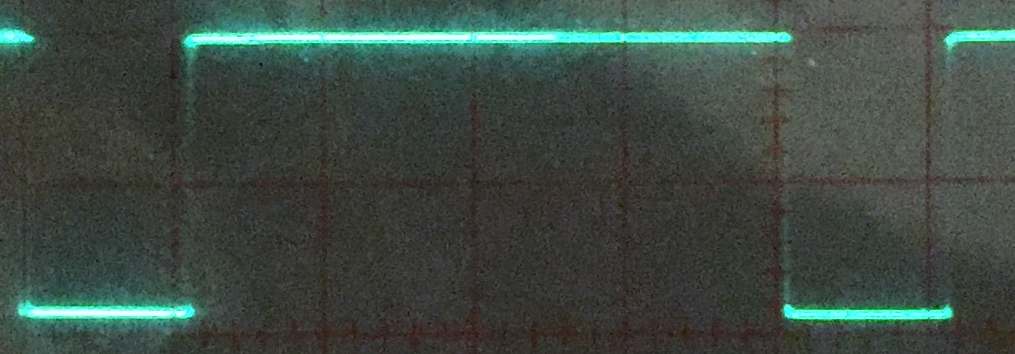
\includegraphics[width=\textwidth]{chapters/hardware-chapters/AC/ac-modulator/custom-hardware/triggering-circuit-output-cropped.png}
	%		\caption{Output from the triggering circuit. Settings: 2 V/div, 2 ms/div.}
	%		\label{fig:triggering-circuit-output}
	%	\end{minipage}
	%	\hfill
	%	\begin{minipage}[b]{0.49\textwidth}
	%		\includegraphics[width=\textwidth]{chapters/hardware-chapters/AC/ac-modulator/custom-hardware/ac-wave-triggering.eps}
	%		\caption{Output form the triggering circuit alongside the incoming AC voltage.}
	%		\label{fig:triggering-circuit-output-2}
	%	\end{minipage}
	%\end{figure}


	\begin{figure}[h]
		\centering
		\begin{minipage}[b]{0.49\textwidth}
			\includegraphics[width=\textwidth]{chapters/hardware-chapters/AC/ac-modulator/custom-hardware/ac-trigger/ac-wave-triggering.eps}
			\caption{Output form the triggering circuit alongside the incoming AC voltage.}
			\label{fig:triggering-circuit-output-2}
		\end{minipage}
		\hfill
		\begin{minipage}[b]{0.49\textwidth}
			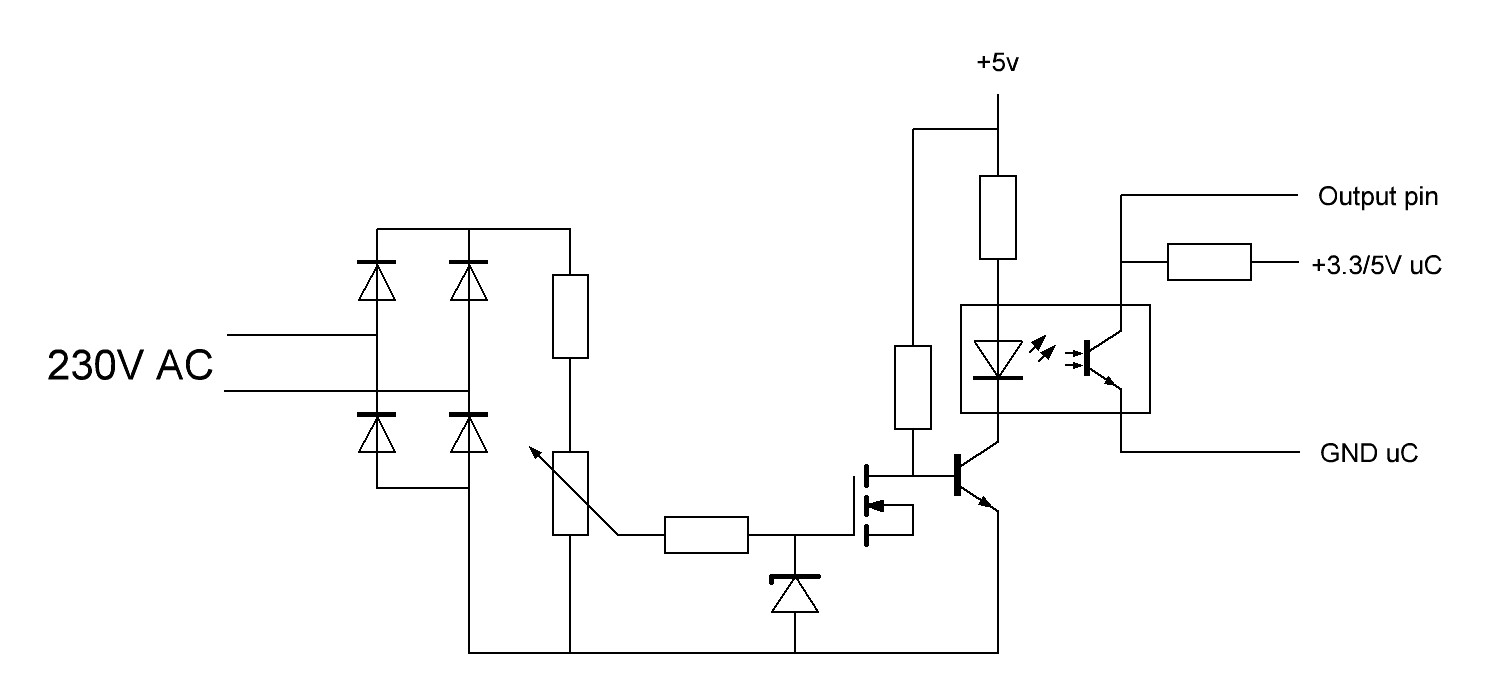
\includegraphics[width=\textwidth]{chapters/hardware-chapters/AC/ac-modulator/custom-hardware/ac-trigger/custom-modulator-trigger.JPG}
		    \caption{Triggering circuit to determine when the voltage is sufficiently high enough to start encoding the ID.}
			\label{fig:custom-modulator-trigger}
		\end{minipage}
	\end{figure}

	In \autoref{fig:triggering-circuit-output-2}, the preset voltage is set at 100 V.
	When more than 100 V is available the LED will emit light and start drawing current.
	At that point, around 1 ms in the figure, the triggering circuit will output a logical `1' to the micro-controller, meaning that the encoding of the ID may start.
	When less than 100 V is available, around 9 ms in the figure, the logical output of the circuit becomes `0', indicating to the micro-controller that it is time to stop encoding the ID, because else information is lost since the LED is not turning on anymore and therefor no longer draws current.
	The same happens for the negative part of the sine wave, except the preset is now $-100$ V.


	From \autoref{fig:triggering-circuit-output-2} it can be deduced that two times 8 ms is available to encode the ID in a period of 20 ms.
	So $\frac{2 \times 8}{20} = 80$ \% of the time is available for modulation, which is two times more than the 230 V AC LED (Figure \ref{fig:commercial-230v-ac-led-on-annotated}) provided.
	%the solution in \autoref{subsubsec:ac-230v-led}
	To transmit the ID, this solution would be two times faster, but it would still take 25 \% more time than in a DC environment.



	In \autoref{fig:custom-modulator-trigger}, the circuit can be seen which signals the micro-controller when the voltage is more or less than the preset voltage. 
	The voltage preset can be set by using a potentiometer.
	The output of the circuit is electrically isolated from the micro-controller by the means of an optocoupler.
	This is done to protect the micro-controller from the high voltage AC in the development stages.